
\section{Luck}
\andyc{Lucas's section}

No change. It's not about the prize, it's the element of luck involved that makes it 50\%. William Cukierski ,Kaggle Competition Admin \\

Having detailed popular methods for prediction and outlined our new methodology that accounts for specific match ups, the final component of this paper addresses the high degree of chance present in NCAA tournaments and consequently prediction for NCAA tournaments.  Specifically we address how sensitivity in a Kaggle style leader board . It's natural to think 2nd place almost won, but how close was 20th place to winning? 

% some verbiage in here... 

To study the effect of luck we take the idea that the 2nd place team almost won and we attempt to quantify `almost'. There are several ways one might consider to conduct a study of this sort, we examine alternate realities where a losing team in a game is treated equally as a winning team in the case of an overtime. We focus only on overtime games because it seems reasonable to consider the fact that these games could have gone either to the victor or the loser. Recalling that the loss function used for scoring of the waggle competition is

\begin{equation}
\sum_{i=1}^n\frac{y_ilog(p_i)+ (1-y_i)log(1-p_i)}{n},
\end{equation}

Where $y_i$ is a binary variable taking value 1 when the team wins and 0 otherwise and $0 \leq p_i \leq 1$ denotes the predicted value for the team in the $i$th game.  
We ask the question how dependent on the characteristics of this particular loss function is the ranking of individual teams? 

To answer this question we studied a couple of possible alternate scoring functions. We consider the following scoring functions: 
 
 \lucasc{Here will be the three eqns here}

\begin{equation}
-log(1-2|.5-p_i|)
\end{equation} 

\begin{equation}
-log(1-|.5-p_i|)
\end{equation} 

\begin{equation}\label{eqn:third_score_function}
-log(1-|y_i-p_i|)
\end{equation} 
Here, for brevity, we only write the part of the loss function multiplied by the $(1-y_i)$ term in the loss function above. Moreover, in Function \ref{eqn:third_score_function}, $y_i \in \{0,.5,1\}$, where now the $0.5$ is the realized value when teams go into overtime. A plot of the different score functions for values $0\leq p_i \leq 1$ is shown in Figure \ref{fig:scoring_functions}.  

\begin{figure}[h]
\centering
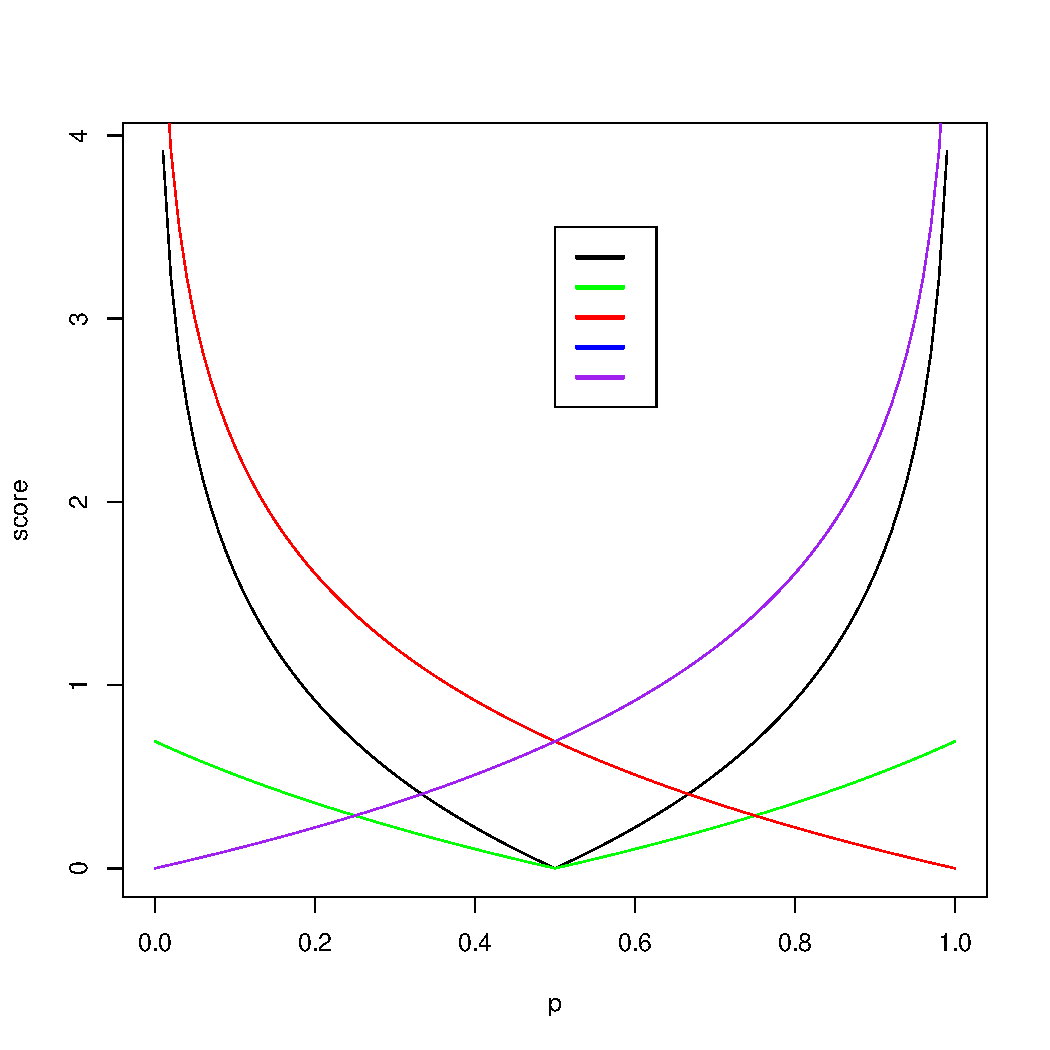
\includegraphics[width=.7\textwidth]{loss_function_plot.pdf}
\caption{A plot of the various loss functions as a function of the prediction $p_i$.  }
\label{fig:scoring_functions}
\end{figure}

